\documentclass[landscape,final,a0paper,fontscale=0.285]{baposter}

\usepackage{calc}
\usepackage{graphicx}
\usepackage{amsmath}
\usepackage{amssymb}
\usepackage{relsize}
\usepackage{multirow}
\usepackage{rotating}
\usepackage{bm}
\usepackage{url}

\usepackage{graphicx}
\usepackage{multicol}

%\usepackage{times}
%\usepackage{helvet}
%\usepackage{bookman}
\usepackage{palatino}

\newcommand{\captionfont}{\footnotesize}

\graphicspath{{images/}{../images/}}
\usetikzlibrary{calc}

\newcommand{\SET}[1]  {\ensuremath{\mathcal{#1}}}
\newcommand{\MAT}[1]  {\ensuremath{\boldsymbol{#1}}}
\newcommand{\VEC}[1]  {\ensuremath{\boldsymbol{#1}}}
\newcommand{\Video}{\SET{V}}
\newcommand{\video}{\VEC{f}}
\newcommand{\track}{x}
\newcommand{\Track}{\SET T}
\newcommand{\LMs}{\SET L}
\newcommand{\lm}{l}
\newcommand{\PosE}{\SET P}
\newcommand{\posE}{\VEC p}
\newcommand{\negE}{\VEC n}
\newcommand{\NegE}{\SET N}
\newcommand{\Occluded}{\SET O}
\newcommand{\occluded}{o}

%%%%%%%%%%%%%%%%%%%%%%%%%%%%%%%%%%%%%%%%%%%%%%%%%%%%%%%%%%%%%%%%%%%%%%%%%%%%%%%%
% Multicol Settings
%%%%%%%%%%%%%%%%%%%%%%%%%%%%%%%%%%%%%%%%%%%%%%%%%%%%%%%%%%%%%%%%%%%%%%%%%%%%%%%%
\setlength{\columnsep}{1.5em}
\setlength{\columnseprule}{0mm}

%%%%%%%%%%%%%%%%%%%%%%%%%%%%%%%%%%%%%%%%%%%%%%%%%%%%%%%%%%%%%%%%%%%%%%%%%%%%%%
%%% Begin of Document
%%%%%%%%%%%%%%%%%%%%%%%%%%%%%%%%%%%%%%%%%%%%%%%%%%%%%%%%%%%%%%%%%%%%%%%%%%%%%%

\begin{document}

%%%%%%%%%%%%%%%%%%%%%%%%%%%%%%%%%%%%%%%%%%%%%%%%%%%%%%%%%%%%%%%%%%%%%%%%%%%%%%
%%% Here starts the poster
%%%---------------------------------------------------------------------------
%%% Format it to your taste with the options
%%%%%%%%%%%%%%%%%%%%%%%%%%%%%%%%%%%%%%%%%%%%%%%%%%%%%%%%%%%%%%%%%%%%%%%%%%%%%%
% Define some colors

%\definecolor{lightblue}{cmyk}{0.83,0.24,0,0.12}
\definecolor{lightblue}{rgb}{0.145,0.6666,1}

%%
\begin{poster}%
  % Poster Options
  {
  % Show grid to help with alignment
  grid=false,
  % Column spacing
  colspacing=1em,
  columns=3,
  % Color style
  bgColorOne=white,
  bgColorTwo=white,
  borderColor=lightblue,
  headerColorOne=black,
  headerColorTwo=lightblue,
  headerFontColor=white,
  boxColorOne=white,
  boxColorTwo=lightblue,
  % Format of textbox
  textborder=roundedleft,
  % Format of text header
  eyecatcher=true,
  headerborder=closed,
  headerheight=0.1\textheight,
%  textfont=\sc, An example of changing the text font
  headershape=roundedright,
  headershade=shadelr,
  headerfont=\Large\bf\textsc, %Sans Serif
  textfont={\setlength{\parindent}{1.5em}},
  boxshade=plain,
%  background=shade-tb,
  background=plain,
  linewidth=2pt
  }
  % Eye Catcher
  {
    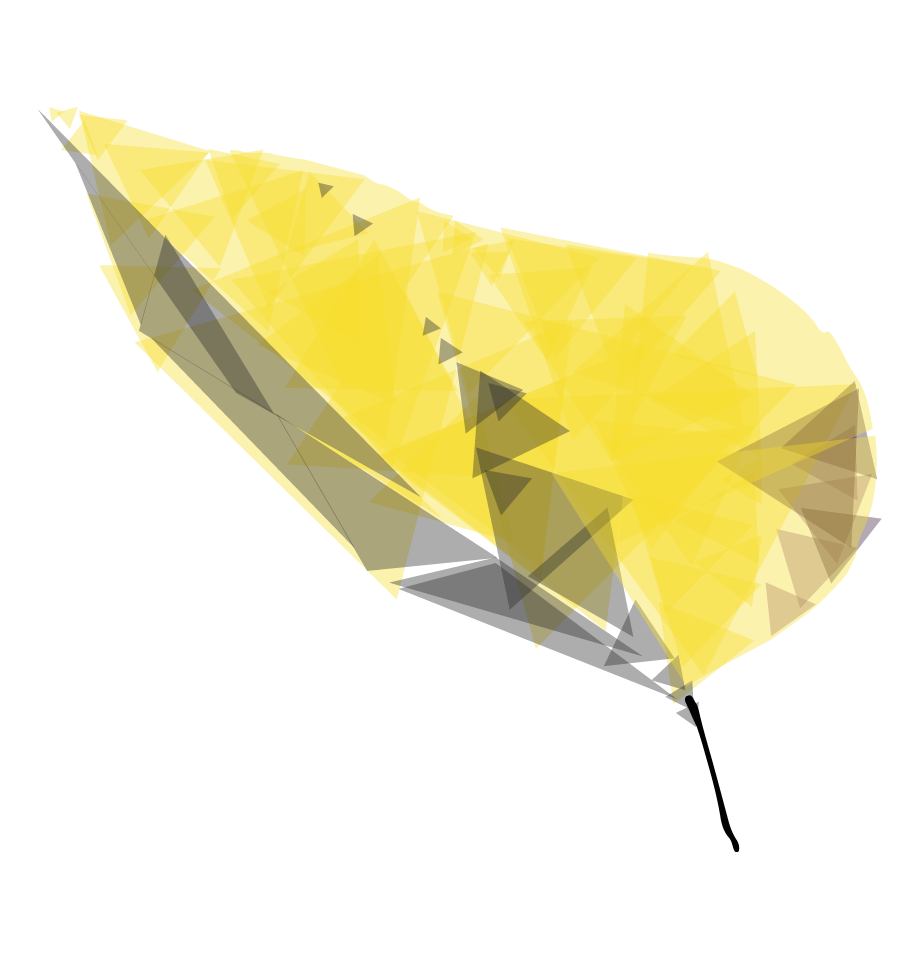
\includegraphics[height=5em]{img/datavyu-leaf-large.png}
  } 
  %Title
  {\bf{Sharing displays and data from vision science research with Databrary} }
  % Authors
  {Rick O. Gilmore \emph{(rick@databrary.org)}, Karen E. Adolph, David S. Millman, Lisa Steiger, and Dylan A. Simon \\
  VSS 2015 -- Poster 26.4031}
  % University logo
  {
    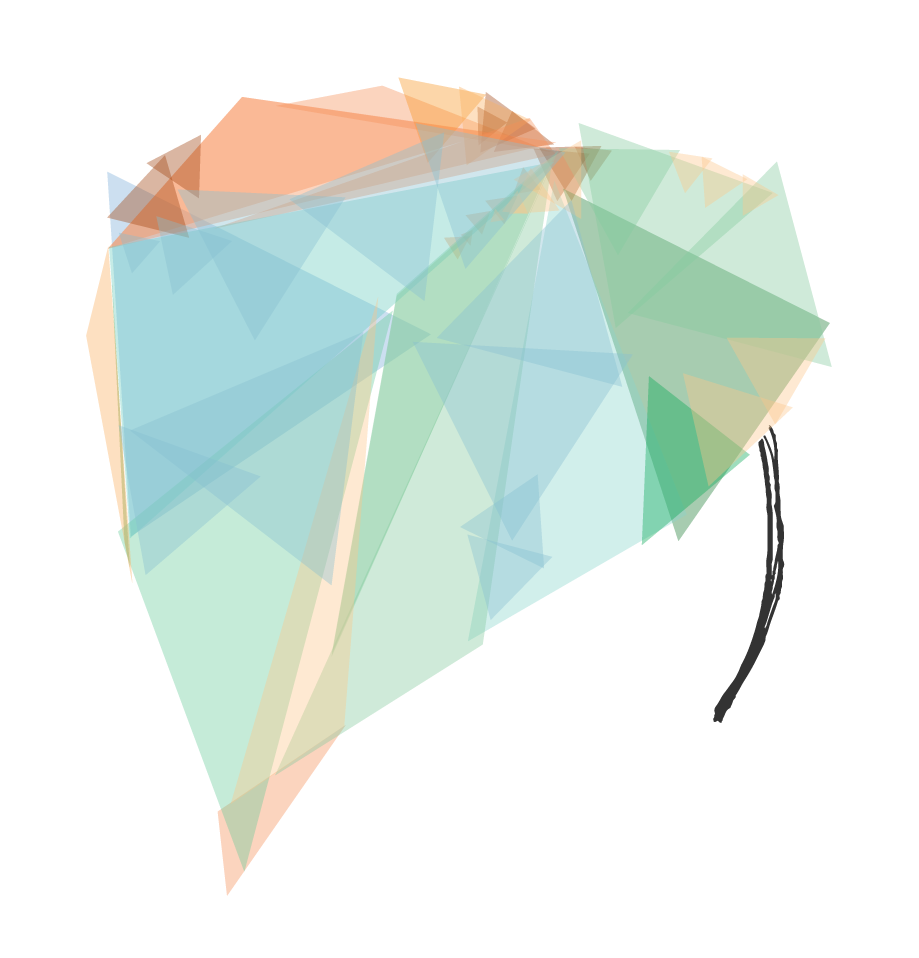
\includegraphics[height=5em]{img/databrary-leaf-large.png}
  }

%%%%%%%%%%%%%%%%%%%%%%%%%%%%%%%%%%%%%%%%%%%%%%%%%%%%%%%%%%%%%%%%%%%%%%%%%%%%%%
%%% Now define the boxes that make up the poster
%%%---------------------------------------------------------------------------
%%% Each box has a name and can be placed absolutely or relatively.
%%% The only inconvenience is that you can only specify a relative position 
%%% towards an already declared box. So if you have a box attached to the 
%%% bottom, one to the top and a third one which should be in between, you 
%%% have to specify the top and bottom boxes before you specify the middle 
%%% box.
%%%%%%%%%%%%%%%%%%%%%%%%%%%%%%%%%%%%%%%%%%%%%%%%%%%%%%%%%%%%%%%%%%%%%%%%%%%%%%

%%%%%%%%%%%%%%%%%%%%%%%%%%%%%%%%%%%%%%%%%%%%%%%%%%%%%%%%%%%%%%%%%%%%%%%%%%%%%%
  \headerbox{Problem}{name=problem,column=0,row=0}{
%%%%%%%%%%%%%%%%%%%%%%%%%%%%%%%%%%%%%%%%%%%%%%%%%%%%%%%%%%%%%%%%%%%%%%%%%%%%%%
      The open sharing of data and workflows from scientific research has gained increasing attention in many fields and has become a priority for research funders. 
      Databrary (databrary.org) is a digital data library specialized for storing and sharing video and research data and metadata. Vision scientists often present temporally varying visual displays to human or non-human animal observers and may collect gaze position, kinematic data, or other physiological recordings simultaneously. 
      Some vision scientists collect identifiable video recordings of participants for use in off-line tagging or coding. 
      Databrary may be especially well suited for these use cases because of the library's focus on uploading, organizing, storing, and sharing research data and metadata collected in the course of behavioral resesearch.
      Databrary has developed policies that enable identifiable information to be shared with the permission of research participants.
 }

%%%%%%%%%%%%%%%%%%%%%%%%%%%%%%%%%%%%%%%%%%%%%%%%%%%%%%%%%%%%%%%%%%%%%%%%%%%%%%
  \headerbox{Privacy \& Security}{name=privacy,column=0,row=1, below=problem}{
%%%%%%%%%%%%%%%%%%%%%%%%%%%%%%%%%%%%%%%%%%%%%%%%%%%%%%%%%%%%%%%%%%%%%%%%%%%%%%
      Videos may contain identifiable information such as faces, voices, and images of places. 
      Databrary ensures that identifiable information can be shared in two ways:
      \begin{itemize}
      \item{\bf{Restricting Access}}

      Only those with independent researcher status at an institution may apply for authorization. 
      Applicants promise to uphold ethical principles and sign an access agreement co-signed by the institution.

      \item{\bf{Securing Permission to Share}}

      Identifiable data may only be shared if participants have given permisssion.
      The Databrary release template may be adapted for specific research protocols.

      \end{itemize}
  }

%%%%%%%%%%%%%%%%%%%%%%%%%%%%%%%%%%%%%%%%%%%%%%%%%%%%%%%%%%%%%%%%%%%%%%%%%%%%%%
  \headerbox{What Can Be Shared}{name=shared,column=1,row=0}{
%%%%%%%%%%%%%%%%%%%%%%%%%%%%%%%%%%%%%%%%%%%%%%%%%%%%%%%%%%%%%%%%%%%%%%%%%%%%%%
    Databrary can house video, audio, PDF, spreadsheet, image, and text-based files (along with associated metadata), as well as executable scripts in Ruby, R and Matlab that facilitate data analysis.
    Video and audio data are transcoded into standard and HTML5-compatible formats, currently H.264+AAC as MP4. Databrary stores other data in native formats (e.g., .doc, .docx, .xls, .xlsx, .txt, .csv, .pdf, .jpg, .png).
  }

%%%%%%%%%%%%%%%%%%%%%%%%%%%%%%%%%%%%%%%%%%%%%%%%%%%%%%%%%%%%%%%%%%%%%%%%%%%%%%
  \headerbox{Technology Stack}{name=stack,column=0,below=privacy}{
%%%%%%%%%%%%%%%%%%%%%%%%%%%%%%%%%%%%%%%%%%%%%%%%%%%%%%%%%%%%%%%%%%%%%%%%%%%%%%
    Databary is built on a PostreSQL database using the Scala Play framework and JavaScript.
    Data are preserved indefinitely in a secure data storage facility at NYU managed by central IT. 
    There is no cost to use the system; an institutional subscription model is under development.
    All code is hosted on GitHub.
  }

%%%%%%%%%%%%%%%%%%%%%%%%%%%%%%%%%%%%%%%%%%%%%%%%%%%%%%%%%%%%%%%%%%%%%%%%%%%%%%
\headerbox{Databrary.org}{name=splash,column=1,span=1,row=0}{
  %%%%%%%%%%%%%%%%%%%%%%%%%%%%%%%%%%%%%%%%%%%%%%%%%%%%%%%%%%%%%%%%%%%%%%%%%%%%%%
  \begin{center}
    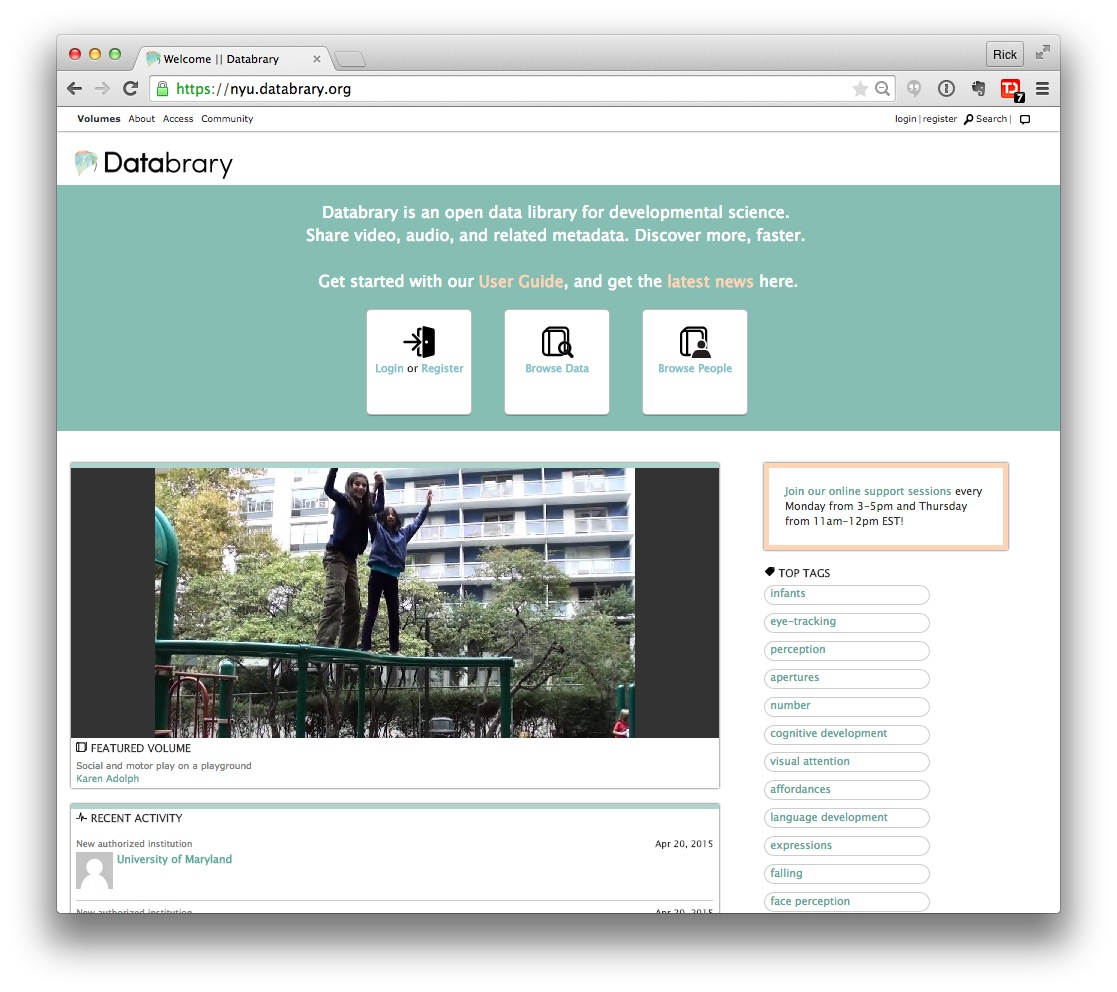
\includegraphics[width=\textwidth]{img/databrary-splash.png}
  \end{center}
  % Databrary's splash page shows a timeline of recent activity, a set of clickable tags that link to studies with those search terms, a featured dataset, and links that enable users to search for data or manage their own data.
}

%%%%%%%%%%%%%%%%%%%%%%%%%%%%%%%%%%%%%%%%%%%%%%%%%%%%%%%%%%%%%%%%%%%%%%%%%%%%%%
\headerbox{Volume/Dataset Page}{name=volume,column=2,span=1,row=0,bottomaligned=splash}{
  %%%%%%%%%%%%%%%%%%%%%%%%%%%%%%%%%%%%%%%%%%%%%%%%%%%%%%%%%%%%%%%%%%%%%%%%%%%%%%
  \begin{center}
  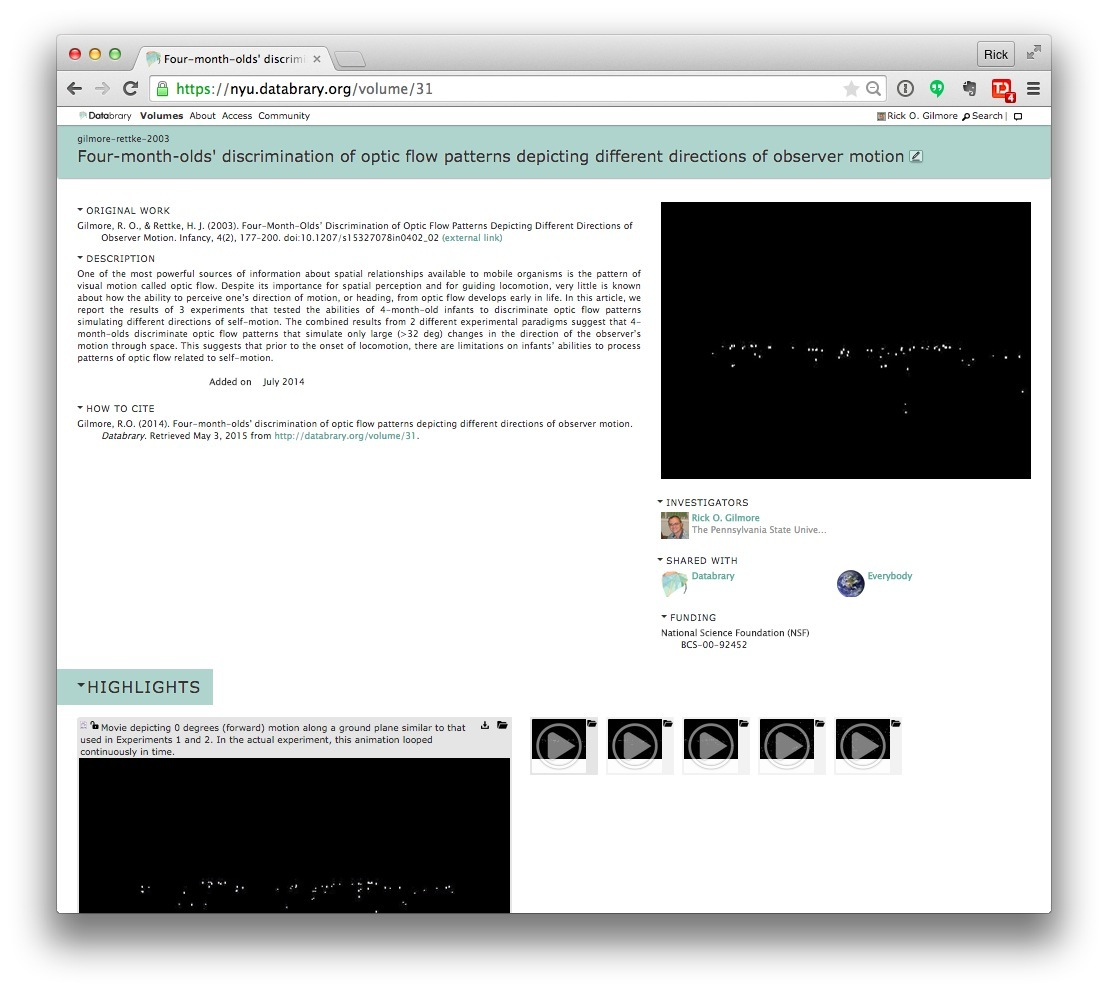
\includegraphics[width=\textwidth]{img/volume-31-new.jpg}
  \end{center}
}

%%%%%%%%%%%%%%%%%%%%%%%%%%%%%%%%%%%%%%%%%%%%%%%%%%%%%%%%%%%%%%%%%%%%%%%%%%%%%%
  \headerbox{Acknowledgments}{name=thanks,column=0,span=2,above=bottom}{
%%%%%%%%%%%%%%%%%%%%%%%%%%%%%%%%%%%%%%%%%%%%%%%%%%%%%%%%%%%%%%%%%%%%%%%%%%%%%%
  Databrary is based on work supported by the National Science Foundation under Grant No. BCS-1238599 and the Eunice Kennedy Shriver National Institute of Child Health and Human Development under Cooperative Agreement U01-HD-076595. 
  Any opinions, findings, and conclusions or recommendations expressed in the material contributed here are those of the author(s) and do not necessarily reflect the views of the National Science Foundation or the Eunice Kennedy Shriver National Institute of Child Health and Human Development.
  }

%%%%%%%%%%%%%%%%%%%%%%%%%%%%%%%%%%%%%%%%%%%%%%%%%%%%%%%%%%%%%%%%%%%%%%%%%%%%%%
\headerbox{Session-level Data Management}{name=data,column=1,span=1,below=splash,above=thanks}{
  %%%%%%%%%%%%%%%%%%%%%%%%%%%%%%%%%%%%%%%%%%%%%%%%%%%%%%%%%%%%%%%%%%%%%%%%%%%%%%
  \begin{center}
    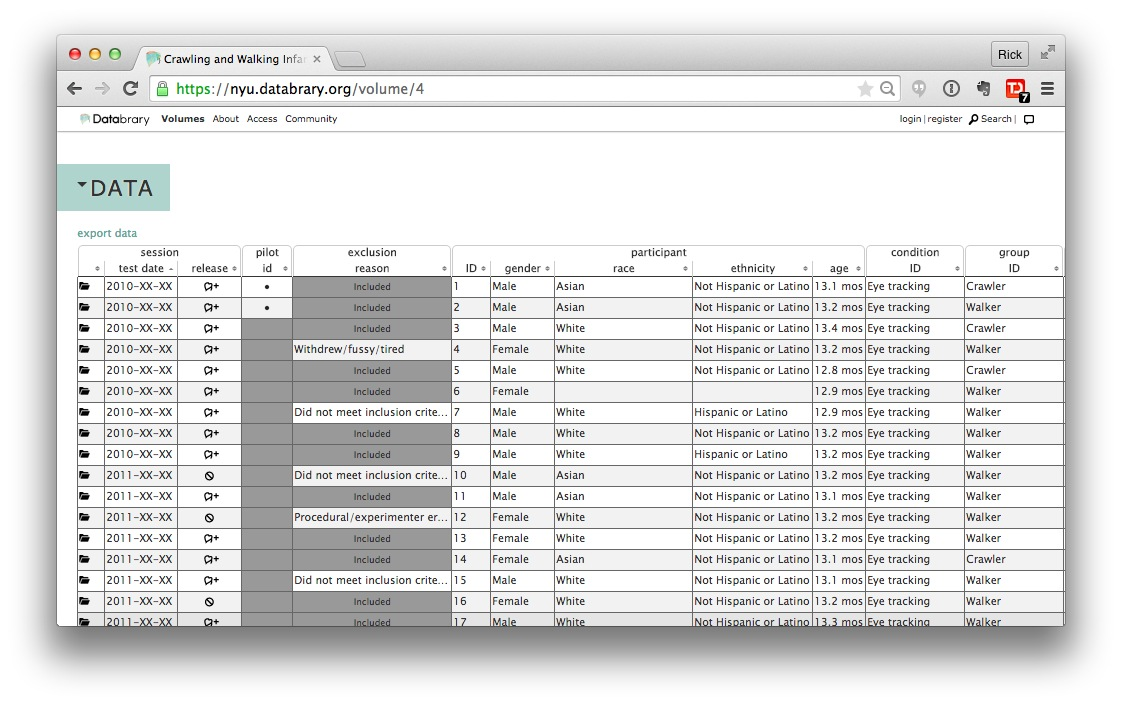
\includegraphics[width=.9\textwidth]{img/spreadsheet.png}
  \end{center}
  % Users may upload video and related data \emph{as they collect it}, recording information about individual data collection sessions such as participant characteristics, sharing permission levels, and study conditions.
}

%%%%%%%%%%%%%%%%%%%%%%%%%%%%%%%%%%%%%%%%%%%%%%%%%%%%%%%%%%%%%%%%%%%%%%%%%%%%%%
\headerbox{Timeline}{name=data,column=2,span=1,row=1,below=volume, above=bottom, aligned=data}{
  %%%%%%%%%%%%%%%%%%%%%%%%%%%%%%%%%%%%%%%%%%%%%%%%%%%%%%%%%%%%%%%%%%%%%%%%%%%%%%
  \begin{center}
  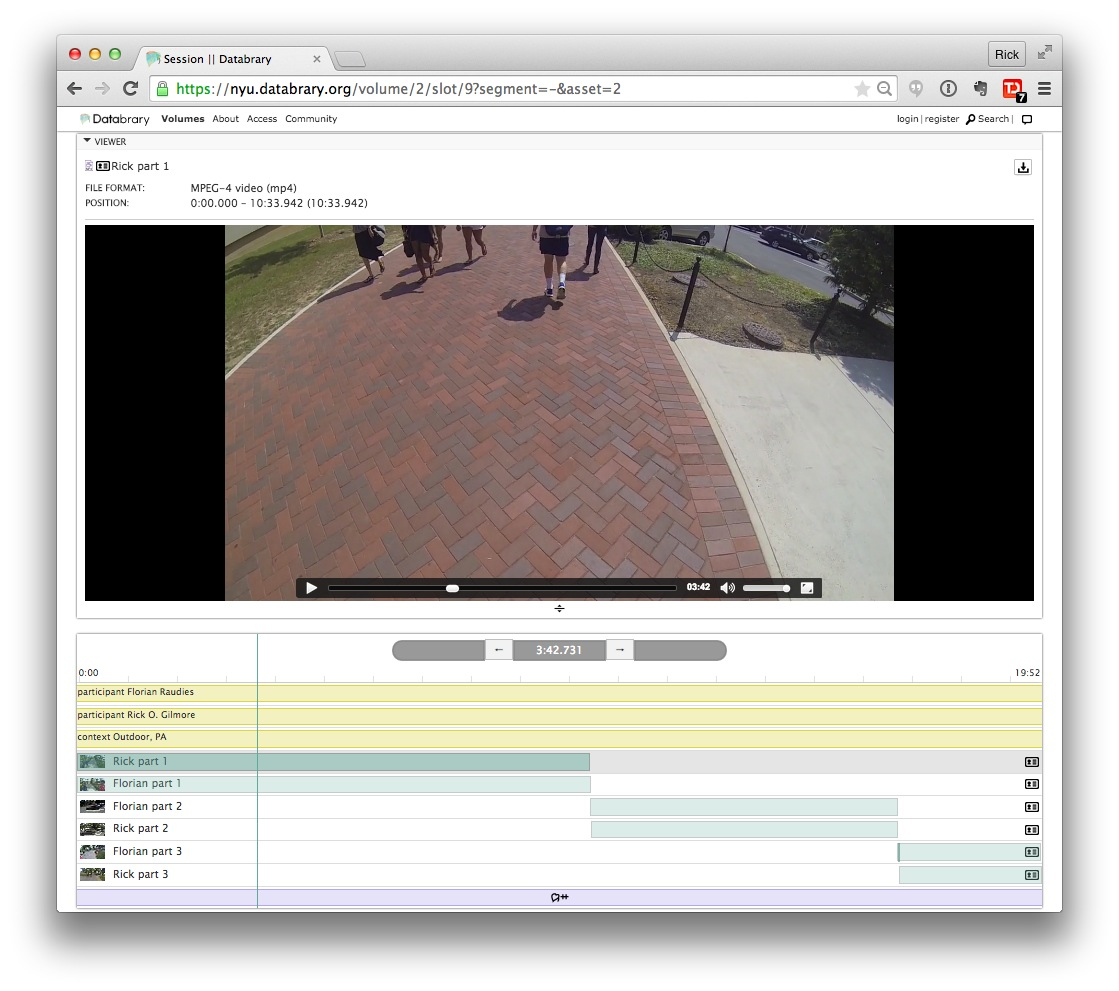
\includegraphics[width=.95\textwidth]{img/timeline.png}
  \end{center}
  % Within a session, data are represented on a timeline that reflects when events occurred. This is particularlly useful for studies with multiple camera views (e.g., eye-tracking) or with combined behavioral and image/display streams.
}

\end{poster}

\end{document}
